
\section{Solution}
\label{sec:auswertung}

\begin{itemize}
    \item[1.]
    In the first execerise we were supossed to write an algorythm to estimate the time evolution of the wavefunction, that solves the Schrödinger equation.
    \begin{itemize}
        \item[a)]
        In the first part were had to non dimensionlize the Schrödinger equation
        \begin{equation}
            i \partial_\tau \Psi = -\partial_\xi ^2 \Psi + \xi ^2 \Psi = \hat{H} \Psi
        \end{equation}
        \FloatBarrier
        \begin{figure}
            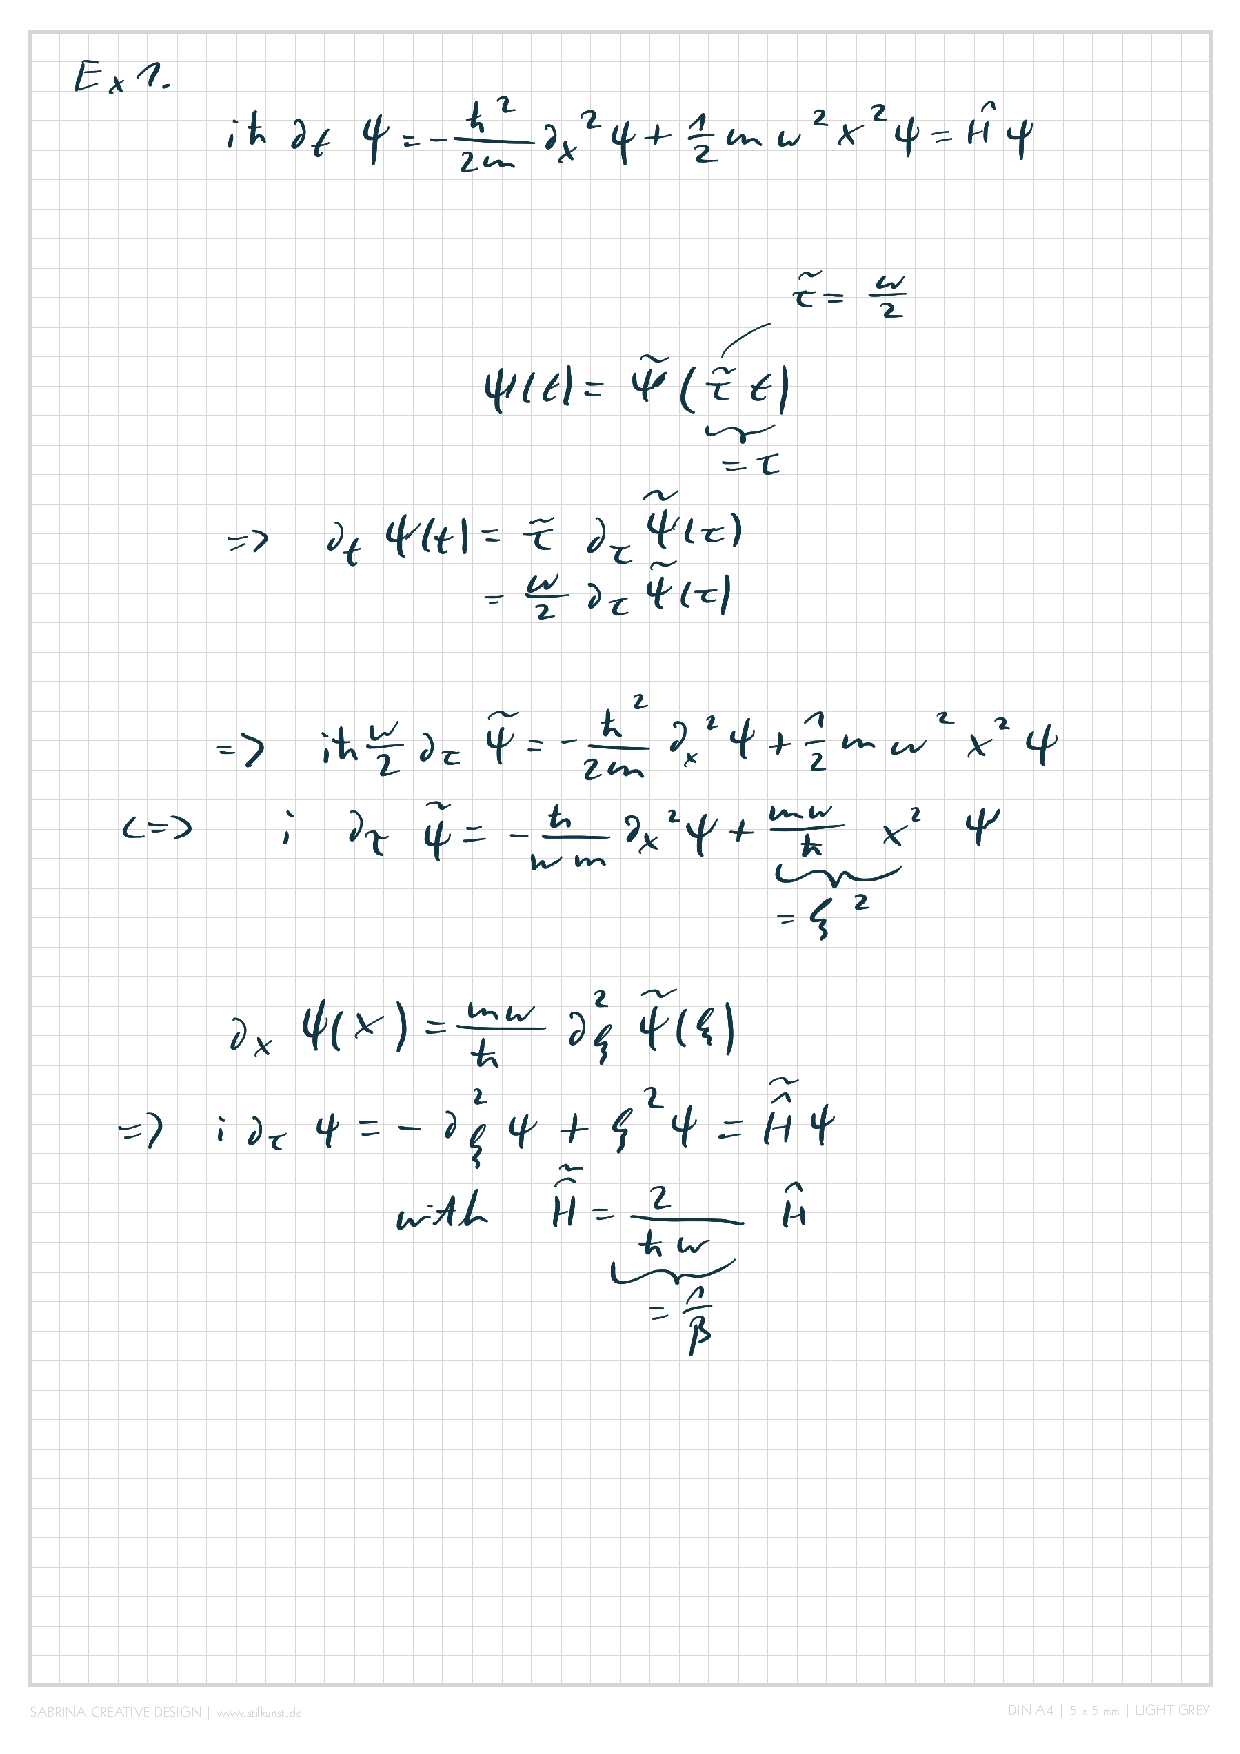
\includegraphics[width=\textwidth]{images/Sheet_5.pdf}
            \caption{The non dimensionilazion of the Schrödinger equation.}
        \end{figure}
        \FloatBarrier
        \item[b)]
        The next step was to implement the Cranck-Nicholson-scheme with a given Hamilton
        \begin{equation}
            H_\text{nm} = - \frac{1}{\Delta \xi ^2} (\delta_\text{n,m-1} + \delta_\text{n,m+1} - 2\delta_\text{n,m}) + \Delta \xi^2 n^2 \delta_\text{n,m} . 
        \end{equation}
        We implemented the scheme in the source file 1.cpp in function "time\_evolution".
        The time evolution matrix is calculated by function "A".
        \item[c)]
        The next part asked us to implement a initial state in form of a gaussian packed 
        \begin{equation}
            \Psi(\xi,0) = \left(\frac{1}{2\pi\sigma}\right)^{1/4} \symup{exp}\left(\frac{-(\xi - \xi_0)^2}{4\sigma}\right)
        \end{equation}
        which was supossed to be normalized.
        So
        \begin{equation}
            1 = \int \symup{d}\xi \xi |\Psi(\xi,0)|^2
        \end{equation}
        which we achieved by we writing the integral as a sum.
        As we work in the numerical regime.
        The implemented version can be found in function "wavefuntion".
        \item[d) + e)]
        In the last to parts we were asked to use the time evolution matrix to estimate the time evolution of the wavefunction up to $t=10$.
        We then had to animate the wavefunction in time.
        The animation can be found as file "schroedinger.gif".
        Note that we also made an animation with a different Hamilton.
        The different Hamilton that we used has a symmetrical potetial around $\xi = 0$, this animation is called "schroedinger\_asitshouldbe.gif".
        For this we changed the $\Delta \xi 2n^2 \delta_\text{n,m}$ to $\Delta \xi 2(n - \frac{10}{\Delta \xi})^2 \delta_\text{n,m}$ which makes the potential symmetrical.

    \end{itemize}
\end{itemize}
\begin{itemize}
    \item[2.]
    \begin{itemize}
        In the second execerise of this sheet we were asked to solve the wave equation in two dimensions.
        \item[a)]
        First we were supossed to discretize the wave equation.
        You can find our solution below 


        \FloatBarrier
        \item[b)]
        \FloatBarrier
        Next we had to analyse the stability of the scheme with a given pertubation.

        \FloatBarrier
        \item[c)]
        \FloatBarrier
        The problem with the given scheme is that it needs not only the current time step $u^{n}$ but also the time step before that $u^{n-1}$.
        This is not problematic after the scheme already started.
        However, for the start it is necessary to use some tricks.
        For this we had a given starting velocity $\frac{\partial u}{\partial t} = 0$.
        With which we could solve the problem:


        \FloatBarrier
        \item[d)]
        \FloatBarrier
        The last step before implementing was to non dimensionlize the wave equation.
        You can find our solution below 
        \FloatBarrier
        \item[e)]
        Now we can implement the whole scheme and solve the wave equation in two dimensions in time.
        We animated our solution, of a wiggeling membrane in a fixed frame, and saved the file as "wave.gif".

    \end{itemize}
\end{itemize}


